\section{Experiments}
  We study the effect of the parameters $N$ and $m$ on the performance of 
  TCP Rapid with the cubic mechanism to create p-streams. The topology in 
  Figure \ref{topology} is used to run a set of experiments with different 
  values of $N$ and $n$. The bottleneck link has a transmission capacity of 
  1 Gbps while the rest of the links have a transmission capacity of 10 Gbps. 
  The end-to-end propagation delay is set to 100 ms. In the experiment we 
  establish 50 Rapid connections sharing the bottleneck link and set their 
  starting time randomly from 60 ms to 165 ms. The experiment was run for 
  500 seconds.
    \begin{figure}[h]
    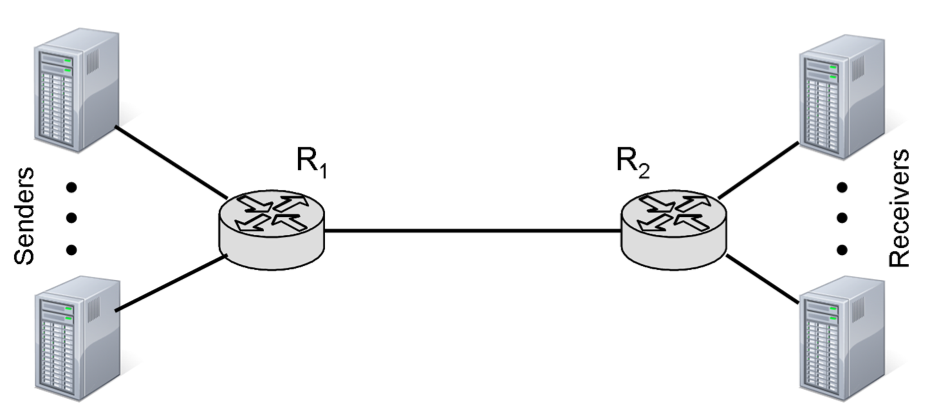
\includegraphics[scale=0.38]{img/topology.png}
    \caption{Experiment topology}
    \label{topology}
  \end{figure}
